\documentclass[a4paper,12pt]{article}


\usepackage{setspace}

\usepackage[T1]{fontenc} % Codificacao da fonte
\usepackage{times} % Definindo a fonte como Times New Roman

\usepackage{fancyhdr}
\pagestyle{fancy}
\lhead{Centro Universitário da FEI}

\rfoot{\thepage} %número da página
\cfoot{\textit{[ELC220] Controle Digital}}

\usepackage[left=2cm,right=2cm,top=2cm,bottom=2cm]{geometry}

\usepackage[utf8]{inputenc}


\usepackage{graphicx}
\usepackage{float}
\usepackage{amsmath}
\usepackage{gensymb}
\usepackage{tikz}
\usepackage{hyperref}
\usetikzlibrary{positioning, arrows, calc}

\begin{document}
	\begin{center}
		\begin{Huge}
			Atividade Parcial
		\end{Huge}
	\end{center}

	\begin{center}
		\centering{\textbf{Gabrielle Magalhães Veras Braga (11.121.557-0)}}\\
		\centering{\textbf{Gustavo Rosell Collado (11.121.526-5)}}\\
		\centering{\textbf{Massiel Blandy Ramón (11.122.397-0)}}\\
		\centering{\textbf{Thiago Travagini Moura (11.121.329-4)}}
	\end{center}
	
	Para ter acesso aos códigos utilizados nessa atividade \href{https://github.com/Thgm01/ELC220-Controle-Digital/tree/main/Atividade_Parcial_01}{Clique Aqui} 
		
	
	\section{Problema 1}
	Uma câmara térmica usada para testes de stress térmico em grandes equipamentos é mostrada na figura 1 com seu respectivo diagrama de blocos simplificado. Considere a unidade de tempo em minuto. A câmara é aquecida por uma linha de vapor que é controlada por uma válvula eletricamente ativa. A abertura da porta afeta a temperatura da câmara e pode ser considerada como um distúrbio. No diagrama de blocos d(t) é um distúrbio causado pela abertura da porta, e(t) é o sinal de entrada do sistema e c(t) a temperatura de saída na câmara térmica.
	

	\begin{figure}[H]
		\centering
		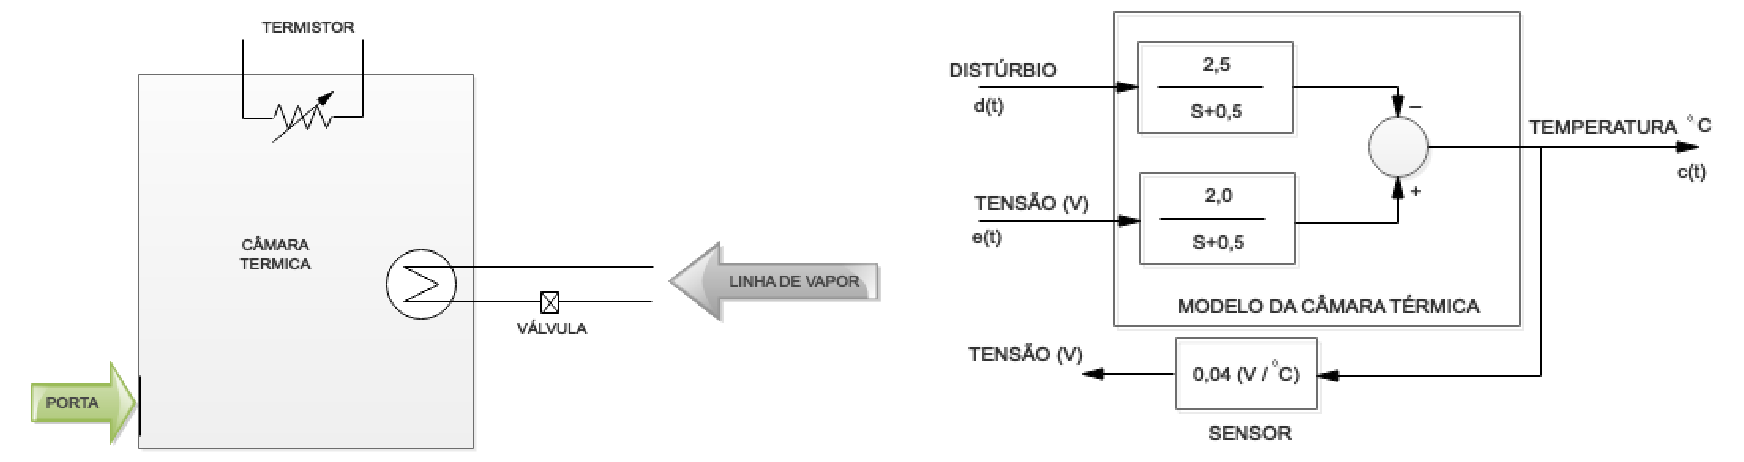
\includegraphics[width=0.9\linewidth]{images/planta_problema1}
		\caption{Câmara térmica para realização de testes de stress em grandes equipamentos e diagrama de blocos simplificado}
		\label{fig:plantaproblema1}
	\end{figure}

	\subsection{Constante de tempo da câmara}
		Para analisarmos qual a constante de tempo do sistema, podemos compara-la a forma genérica da função de sua respectiva ordem, onde nesse caso é um sistema de primeira ordem. Como mostra a equação abaixo é possível obter qual a constante de tempo.
	
		\begin{equation}
			\left.
			\begin{array}{c}
				\displaystyle G(s) = \frac{K}{s+a} \\[20pt]
				\displaystyle \tau = \frac{1}{a}
			\end{array}
			\right\}
			\quad \tau = \frac{1}{0,5} = 2
		\end{equation}
	
		Portanto para câmara proposta a constante de tempo $\tau$ é 2 minutos, portanto o tempo de subida desse ($T_s$) sistema será $4 \cdot \tau = 8$ minutos.
	
	\subsection{Resposta da câmara com condição inicial zero e sem distúrbio}
		Considerando a porta da câmara fechada (sem distúrbio) e com condição inicial 0\degree C, sendo a entrada de sinal um degrau de amplitude cinco tem-se então:
		

		\begin{gather}
			C(s) = \frac{2,0}{s+0,5} \cdot \frac{5,0}{s} = \frac{10,0}{s^2 + 0,5s} = \frac{20}{s} - \frac{20}{s+0,5} \\[20pt]
			c(t) = \mathcal{L}^{-1} \{ C(s) \} = 20 - 20e^{-0,5t}
		\end{gather}
	
		Utilizando o \textit{MATLAB} foi obtido o seguinte gráfico:
		
		\begin{figure}[H]
			\centering
			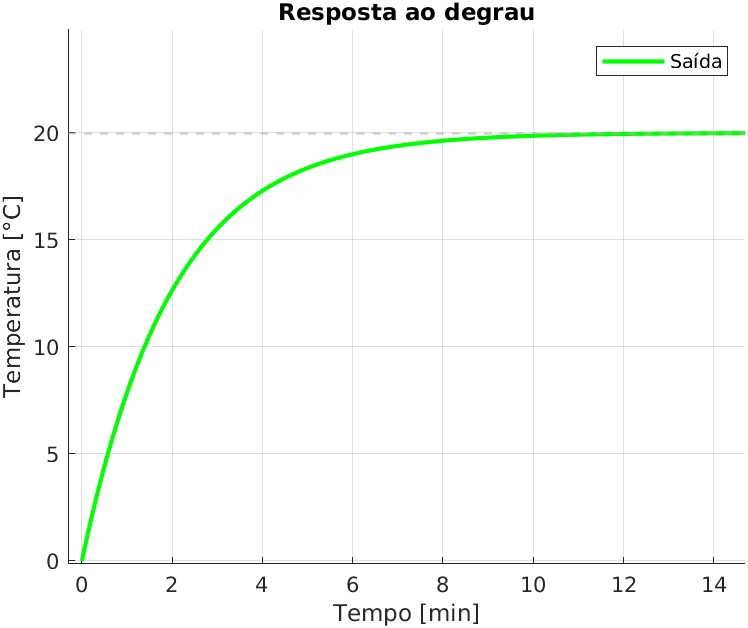
\includegraphics[width=0.5\linewidth]{images/respb.png}
			\caption{Resposta do sistema para um degrau de amplitude 5}
			\label{fig:resposta_b}
		\end{figure}
	
		É possível observar que para essa entrada degrau de amplitude 5 o sistema, para $t$ tendendo ao infinito, estabiliza em 20\degree C.
		
	\subsection{Resposta da câmara com condição inicial 25\degree C e sem distúrbio}
		Sendo feita o mesmo procedimento que o item anterior, porém adicionando uma condição inicial, pode-se dizer que a única mudança será:
		
		\begin{equation}
			c(t) = c_{Anterior}(t) + x_0 \rightarrow c(t) = 45 - 20e^{-0,5t}
		\end{equation}
	
		E com essa equação tem-se o seguinte gráfico.
		
		\begin{figure}[H]
			\centering
			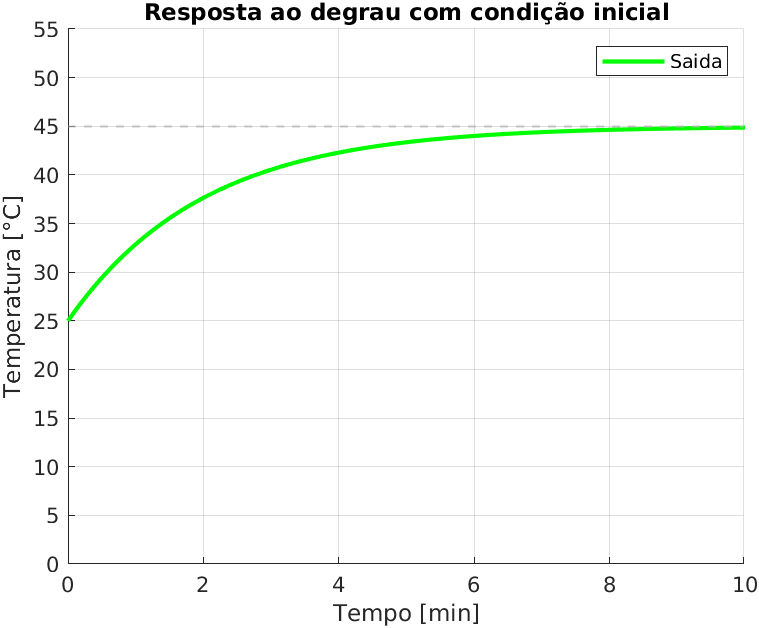
\includegraphics[width=0.5\linewidth]{images/respc.png}
			\caption{Resposta do sistema para um degrau de amplitude 5 e $25 \celsius$ como condição inicial}
			\label{fig:resposta_c}
		\end{figure}
	
	\subsection{Resposta da câmara com condição inicial 25\degree C e com distúrbio continuo}
		Nesse novo cenário é estudado como se comporta a planta para uma entrada degrau de amplitude 5, com condição inicial de 25\degree C e para um distúrbio com uma entrada de degrau unitário após 2 minutos do inicio, tem-se que:
		
		\begin{gather}
			C(s) = G(s) \cdot E(s) - G_d(s) \cdot D(s)  + X_0(s)\\[20pt]
			C(s) = \frac{2,0}{s+0,5} \cdot \frac{5,0}{s} - \frac{2,5}{s+0,5} \cdot \frac{e^{-2s}}{s} + X_0(s) \\[20pt]
			c(t) = \mathcal{L}^{-1} \{ C(s) \} = 20 - 20e^{-0,5t} - (5 - 5e^{-0,5(t-2)})u(t-2) + 25 \\[20pt]
			c(t) = 45 - 20e^{-0,5t} - (5 - 5e^{-0,5(t-2)})u(t-2)
		\end{gather}
	
		Para essas condições a resposta do sistema foi:
		
		\begin{figure}[H]
			\centering
			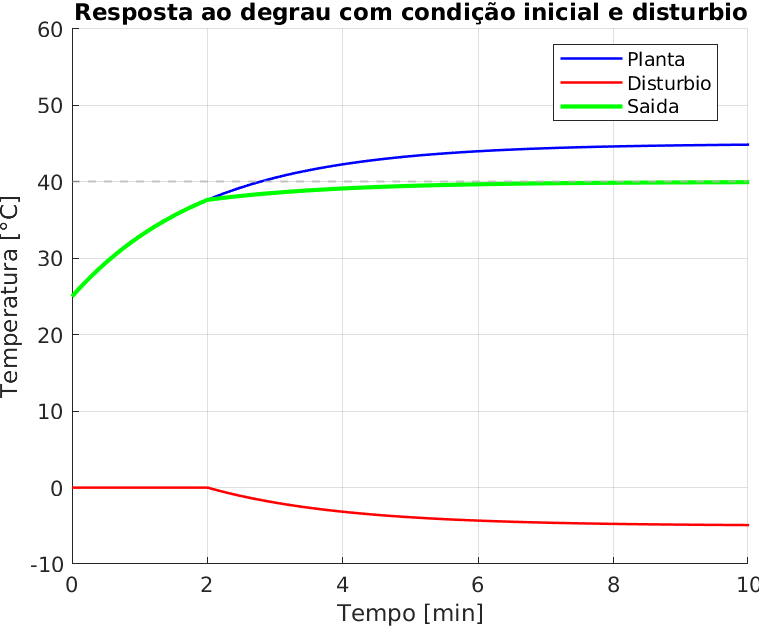
\includegraphics[width=0.5\linewidth]{images/respd.png}
			\caption{Resposta do sistema adicionando um distúrbio}
						
			\label{fig:resposta_d}
		\end{figure}
	
		Do gráfico é possível observar o momento em que o distúrbio começa, em 2 minutos, e o valor final desse distúrbio que é de -5\degree C.
		
	\subsection{Resposta da câmara com condição inicial 25\degree C e com distúrbio finito}
		Nesse ultimo cenário é o mesmo utilizado acima porém com a interrupção do distúrbio apos 12 minutos do seu inicio portanto para obtermos $c(t)$ basta adicionarmos essa interrupção na resposta anterior e a função sera:
		
		\begin{equation}
			c(t) = 45 - 20e^{-0,5t} - (5 - 5e^{-0,5(t-2)})u(t-2) + (5 - 5e^{-0,5(t-14)})u(t-14)
		\end{equation}
	
		E sua resposta foi:
		
		\begin{figure}[H]
			\centering
			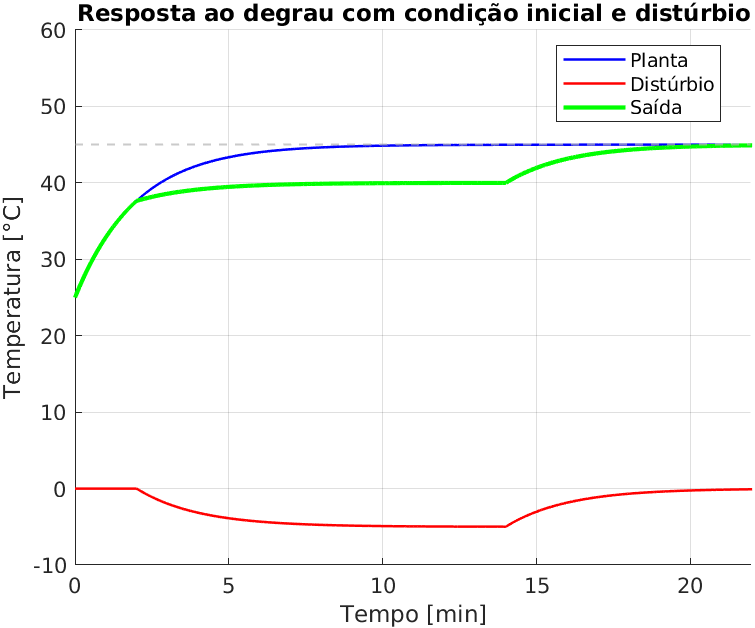
\includegraphics[width=0.5\linewidth]{images/respe.png}
			\caption{Resposta do sistema adicionando um distúrbio temporário}
			\label{fig:resposta_e}
		\end{figure}
	
	\section{Problema 2}
		A figura \ref{fig:plantaproblema2} mostra o sistema de controle de temperatura da câmara térmica do problema 1.
		
		\begin{figure}[H]
			\centering
			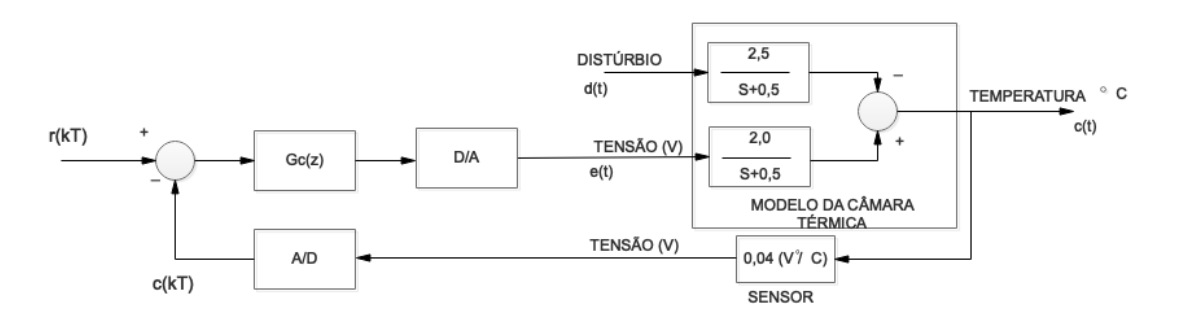
\includegraphics[width=0.9\linewidth]{images/planta_problema2.png}
			\caption{Sistema de controle de temperatura de uma câmara térmica}
			\label{fig:plantaproblema2}
		\end{figure}
	
		\subsection{Função de transferência no domínio z}	
			Para obter a função de transferência no domínio z, é necessário inicialmente realizar algumas modificações nas disposições no diagrama de bloco, para viabilizar a construção das funções de transferências, assim como mostra a figura \ref{fig:diagrama_palnta2_final}.


\begin{figure}[h]
    \centering
    \begin{tikzpicture}[
        block/.style={draw, rectangle, minimum width=1.5cm, minimum height=1cm, align=center},
        sum/.style={draw, circle, node distance=1cm, inner sep=1pt, minimum size=0.5cm},
        node distance=1cm, >=latex]
        
        % Nós do diagrama
        \node (sum) [sum, xshift=0.2cm] {};  % Subtrator
        \node (Gc) [block, right=of sum] {\small$G_c(z)$};
        \node (H) [block, right=of Gc] {\small$H(z)$};
        \node (Gd) [block, above=of sum, xshift=-1.5cm] {\small$\frac{G_d(z)}{G_c(z) \cdot H(z)}$}; % Bloco deslocado para a esquerda
        \node (s) [block, right=of H] {\small$Sensor$};
        \node (sinv) [block, right=of s] {\small$\frac{1}{Sensor}$};
        
        % Nós de entrada e saída
        \node (r) [left=of sum] {\small$R(z)$};
        \node (c) [right=of sinv] {\small$C(z)$};
        \node (d) [left=of Gd] {\small$D(z)$};
        
        % Conexões
        \draw[->] (r) -- node[pos=0.9, above] {\small$+$} (sum.west);
        \draw[->] (sum) -- (Gc);
        \draw[->] (Gc) -- (H);
        \draw[->] (H) -- (s);
        \draw[->] (s) -- (sinv);
        \draw[->] (sinv) -- (c);
        \draw[->] (d) -- (Gd);
        
        % Realimentação
        \node (fb) [coordinate, below=of Gc] {};
        \draw[->] (s) -- ++(1, 0) |- (fb) -| node[pos=0.85, above, xshift=2.5mm] {\small$-$} (sum);
        
		\draw[->] (Gd.east) -| node[pos=0.95, above, , xshift=0.2cm] {\small$-$} (sum.north);

    \end{tikzpicture}
    \caption{Diagrama de blocos da câmara térmica}
    \label{fig:diagrama_palnta2_final}
\end{figure}
			Agora com o sistema modificado é necessário converter a planta e os conversores para o domínio z. Com $T=0,6$ min temos:
					
		
			\begin{equation}
				\left.
				\begin{array}{c}
					\displaystyle H(z) = (1 - z^{-1}) \cdot Z\left[\frac{G(s)}{s}\right] \\[20pt]
					
					\displaystyle Z\left[\frac{G(s)}{s}\right] = Z\left[\frac{2,0}{s(s+0,5)}  \right] = 4 \cdot Z\left[\frac{0,5}{s(s+0,5)}\right] = 4 \cdot \frac{(1 - e^{-0,5T})z}{(z-1)(z-e^{-0,5T})} \\[20pt]
					\displaystyle H(z) = \frac{z-1}{z} \cdot 4 \cdot \frac{(1 - e^{-0,5T})z}{(z-1)(z-e^{-0,5T})} = \frac{4(1 - e^{-0,5T})}{(z-e^{-0,5T})} = \frac{1,036}{(z-0,741)}
				\end{array}
				\right.
				\quad 
				\label{eq:hz06}
			\end{equation}
			
			Portanto tem-se um sistema representado pelo seguinte diagrama de blocos.


		\begin{figure}[h]
		    \centering
		    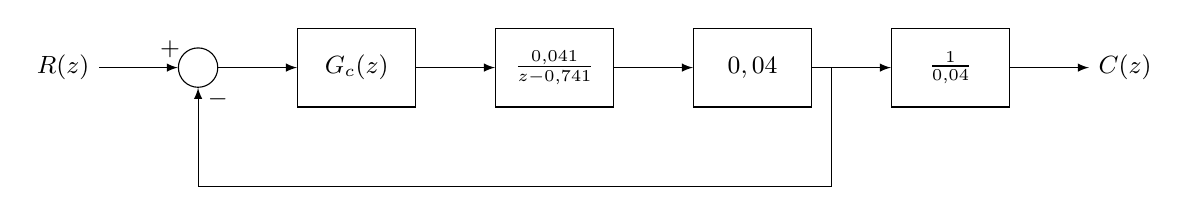
\begin{tikzpicture}[
		        block/.style={draw, rectangle, minimum width=1.5cm, minimum height=1cm, align=center},
		        sum/.style={draw, circle, node distance=1cm, inner sep=1pt, minimum size=0.5cm},
		        node distance=1cm, >=latex]
		        
		        % Nós do diagrama
		        \node (sum) [sum] {};  % Subtrator
		        \node (Gc) [block, right=of sum] {\small$G_c(z)$};
		        \node (H) [block, right=of Gc] {\small $\frac{0,041}{z - 0,741}$};
		        \node (s) [block, right=of H] {\small $0,04$};
              	\node (sinv) [block, right=of s] {\small$\frac{1}{0,04}$};
		        
		        
		        % Nós de entrada e saída
		        \node (r) [left=of sum] {\small$R(z)$};
		        \node (c) [right=of sinv] {\small$C(z)$};
		        
		        % Conexões
		        \draw[->] (r) -- node[pos=0.9, above] {\small$+$} (sum.west);
		
		        \draw[->] (sum) -- (Gc);
		        \draw[->] (Gc) -- (H);
		        \draw[->] (H) -- (s);
		        \draw[->] (s) -- (sinv);
		        \draw[->] (sinv) -- (c);
		        
		        \node (fb) [coordinate, below=of Gc] {};
				\draw[->] (s) -- ++(1, 0) |- (fb) -| node[pos=0.85, above, xshift=2.5mm] {\small$-$} (sum) ;
		    \end{tikzpicture}
		    \caption{Diagrama de blocos da câmara térmica sem distúrbio}
		\end{figure}
			
			E a função de transferência de malha fechada será igual:
			
			\begin{equation}
				\left.
				\begin{array}{c}
					\displaystyle \frac{C(z)}{R(z)} = \frac{G_C(z) \cdot \displaystyle \frac{1,036}{(z-0,741)} \cdot 0,04}{1 + \cdot G_C(z) \cdot \displaystyle \frac{1,036}{(z-0,741)} \cdot 0,04} \cdot \frac{1}{0,04} = \frac{G_C(z) \cdot 1,036}{z - 0,741 + G_C(z) \cdot 0,041}
				\end{array}
				\right.
				\quad 
				\label{eq:ftma}
			\end{equation}
		
		\subsection{Distúrbio no domínio z}
			Visualizando a figura \ref{fig:diagrama_planta2_disturbio} e admitindo a entrada $r(kT)=0$, é possível extrair a temperatura $c(t)$ quando há um distúrbio com uma entrada de degrau unitário tem-se o seguinte diagrama de blocos.
			
			\begin{figure}[h]
			    \centering
			    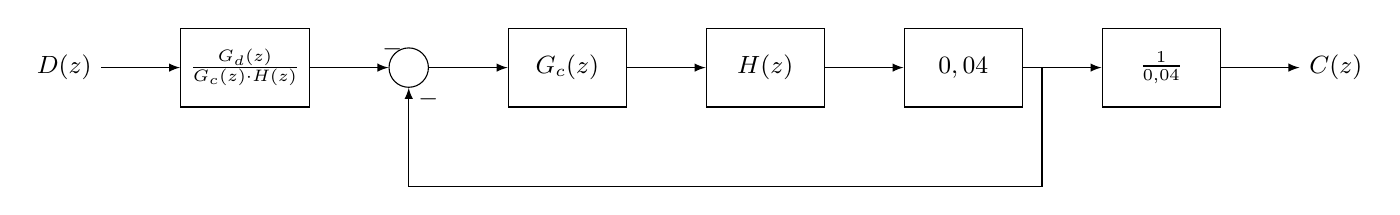
\begin{tikzpicture}[
			        block/.style={draw, rectangle, minimum width=1.5cm, minimum height=1cm, align=center},
			        sum/.style={draw, circle, node distance=1cm, inner sep=1pt, minimum size=0.5cm},
			        node distance=1cm, >=latex]
			        
			        % Nós do diagrama
			        \node (sum) [sum, xshift=0.2cm] {};  % Subtrator
			        \node (Gc) [block, right=of sum] {\small$G_c(z)$};
			        \node (H) [block, right=of Gc] {\small$H(z)$};
			        \node (Gd) [block, left=of sum] {\small$\frac{G_d(z)}{G_c(z) \cdot H(z)}$}; % Bloco deslocado para a esquerda
   			        \node (s) [block, right=of H] {\small$0,04$};
			        
			        \node (sinv) [block, right=of s] {\small$\frac{1}{0,04}$};
			        
			        % Nós de entrada e saída
			        \node (c) [right=of sinv] {\small$C(z)$};
			        \node (d) [left=of Gd] {\small$D(z)$};
			        
			        % Conexões
			        \draw[->] (sum) -- (Gc);
			        \draw[->] (Gc) -- (H);
			        \draw[->] (H) -- (s);
			        \draw[->] (s) -- (sinv);
			        \draw[->] (sinv) -- (c);
			        \draw[->] (d) -- (Gd);
			        
			        % Realimentação
			        \node (fb) [coordinate, below=of Gc] {};
			        \draw[->] (s) -- ++(1, 0) |- (fb) -| node[pos=0.85, above, xshift=2.5mm] {\small$-$} (sum);
			        
					\draw[->] (Gd) -- node[pos=0.85, above, , xshift=0.2cm] {\small$-$} (sum);
			
			    \end{tikzpicture}
			    \caption{Diagrama de blocos do distúrbio}
			    \label{fig:diagrama_planta2_disturbio}
			\end{figure}
			
			
			\begin{equation}
				\left.
				\begin{array}{c}
					\displaystyle C_d(z) = -\frac{G_d(z)}{G_c(z) \cdot H(z)} \cdot \frac{G_c(z) \cdot H(z) \cdot 0,04}{1 + G_c(z) \cdot H(z) \cdot 0,04} \cdot \frac{1}{0,04} = - \frac{G_d(z)}{1 + G_c(z) \cdot H(z) \cdot 0,04} \cdot D(z) \\[20pt]
					
					\displaystyle G_d(z) = Z\left[\frac{2,5}{s+0,5} \right] = 2,5 \cdot Z\left[\frac{1}{s+0,5} \right] = \frac{2,5z}{z-0,741}  \\[20pt]
					
					\displaystyle C_d(z) = -\frac{2,5z}{z-0,741} \cdot \frac{z-0,741}{z-0,741 + G_c\cdot 0,041} \cdot  D(z) \rightarrow \\[20pt]
					
					\displaystyle \rightarrow C_d(z) = - \frac{2,5z}{z-0,741 + G_c\cdot 0,041} \cdot D(z)
					
				\end{array}
				\right.
				\quad 
			\end{equation}
			
			
			
%			\begin{equation}
%				\left.
%				\begin{array}{c}
%					\displaystyle G_d(z) = Z\left[\frac{2,5}{s+0,5} \cdot 0,04\right] \cdot \frac{1}{H(z)}  \\[20pt]
%					
%					\displaystyle Z\left[\frac{2,5}{s+0,5} \cdot 0,04\right] = 2,5 \cdot 0,04 \cdot Z\left[\frac{1}{s+0,5} \right] = \frac{0,1z}{z-0,741} \\[20pt]
%					
%					\displaystyle G_d(z) = \frac{0,1z}{z-0,741} \cdot \frac{(z-0,741)}{0,041} = 2,439z
%					
%				\end{array}
%				\right.
%				\quad 
%			\end{equation}
			
			E para uma entrada degrau unitário tem-se:
			
			\begin{equation}
				\left.
				\begin{array}{c}
					\displaystyle \rightarrow C_d(z) = - \frac{2,5z}{z-0,741 + G_c\cdot 0,041} \cdot \frac{z}{z-1} \cdot z^{-n} \rightarrow \\[20pt]
					
					\displaystyle \rightarrow C_d(z) = - \frac{2,5z^{2-n}}{(z-0,741 + G_c\cdot 0,041)(z-1)} \\[20pt]
				\end{array}
				\right.
				\quad 
			\end{equation}
						
			
		\subsection{Expressão completa do sistema}
			Para obter a expressão completa do sistema é necessário considerado uma entrada $r(kT)$ genérica e um distúrbio que ocorre num instante n. Dessa forma tem-se:
			
			\begin{equation}
				\left.
				\begin{array}{c}
					\displaystyle C(z) = \frac{G_C(z) \cdot 1,036}{z - 0,741 + G_C(z) \cdot 0,041} \cdot Z\left[r(kT)\right] - \frac{2,5z^{2-n}}{(z-0,741 + G_c\cdot 0,041)(z-1)}
				\end{array}
				\right.
				\quad 
			\end{equation}
			
		\subsection{Cenário 1}
		
			Admitindo um período de amostragem $T = 0,6$ min e $Gc(z) = 1,0$, a equação de diferenças para c(kT) quando é aplicado um degrau r(kT) = 0,4 h(kT) resulta em:
			
			\begin{equation}
				\left.
				\begin{array}{c}
					\displaystyle C(z) = \frac{1,0 \cdot 1,036}{z - 0,741 + 1,0 \cdot 0,041} \cdot Z\left[r(kT)\right] = \frac{1,036\cdot 0,4}{z - 0,7} \cdot H(z)
				\end{array}
				\right.
				\quad 
			\end{equation}
			
			Normalizando tem-se:
			
			\begin{equation}
				\left.
				\begin{array}{c}
					\displaystyle C(z) = \frac{0,414}{z - 0,7} \cdot H(z) = \frac{0,414 \cdot z^{-1} \cdot H(z)}{1 - 0,7 \cdot z^{-1}}  \rightarrow \\[20pt]
					\rightarrow \displaystyle c(kT) = 0,7\cdot c[(k-1)T] + 0,414 \cdot h[(k-1)T]
				\end{array}
				\right.
				\quad 
			\end{equation}
			
			Para se obter qual o valor, em temperatura, para uma entrada degrau com amplitude de 0,4, basta admitir que para esse valor final o erro deve ser nulo portanto:
			
			\begin{equation}
				\left.
				\begin{array}{c}
					\displaystyle e(t)= r(t) - c(t) = 0 \rightarrow c(t) \cdot 0,04 = r(t) \rightarrow c(t) = \frac{0,4}{0,04} = 10 \celsius
				\end{array}
				\right.
				\quad 
			\end{equation}
			
			Utilizando também o teorema do valor final tem-se:
			\begin{equation}
				\left.
				\begin{array}{c}
					\displaystyle \lim_{k \to \infty}f(k) = \lim_{z \to 1}\left[(1-z^{-1})F(z) \right] \rightarrow \lim_{k \to \infty}f(k) = \lim_{z \to 1}\left[ \frac{z-1}{z} \cdot \frac{1,036}{z - 0,7} \cdot 0.4 \cdot \frac{z}{z-1}  \right] \rightarrow \\[20pt]
					
					\displaystyle \rightarrow \lim_{k \to \infty}f(k) =  \lim_{z \to 1}\left[  \frac{0,414}{z - 0,7}  \right] = 1,38 \celsius
				\end{array}
				\right.
				\quad 
			\end{equation}
			
			Nessa situação temos um sistema estável porém com erro de aproximadamente 86,2\%. Utilizando o MATLAB se obtém o gráfico como mostra a figura \ref{fig:resp_2_4}.
			

			\begin{figure}[H]
				\centering
				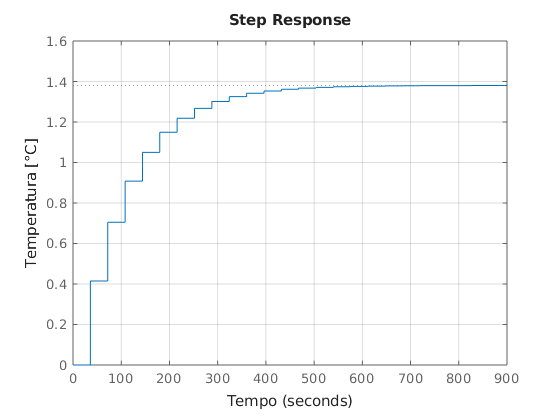
\includegraphics[width=0.6\linewidth]{images/resp2d.png}
				\caption{Resposta do sistema com $T+0,6$, $G_c(z)=1,0$ e $r(kT) = 0,4 h(kT)$}
				\label{fig:resp_2_4}
			\end{figure}
			
		\subsection{Erro cenário 1}
			
			\begin{equation}
				\left.
				\begin{array}{c}
					\displaystyle e(kT) = r(kT) - c(kT) \rightarrow \\[20pt]
					\displaystyle \rightarrow e(kT) = r(kT) - (0,7\cdot c[(k-1)T] + 0,414 \cdot h[(k-1)T]) \rightarrow \\[20pt]
					\displaystyle \rightarrow e(kT) = r(kT) - 0,7 \cdot c[(k-1)T] - 0,414\cdot h[(k-1)T]
				\end{array}
				\right.
				\quad 
			\end{equation}
			
		\subsection{Sistema com ganho infinito}
			Observando a equação \ref{eq:ftma} fica visível que os polos do sistema tem relação direta com o controlador, para um valor de K muito alto o polo do sistema estará fora do circulo de raio unitário do plano z, portanto esse sistema sera instável para uma entrada de degrau unitário.
		
		\subsection{Alterando o período de amostragem}
			Supondo um período de amostragem de $T=6$ mim é necessário refazer alguns cálculos sendo inicialmente o calculo de $H(z)$ realizado na equação \ref{eq:hz06}.
			%TODO: Continuar daqui 
			\begin{equation}
			\left.
			\begin{array}{c}
				\displaystyle H(z) = (1 - z^{-1}) \cdot Z\left[\frac{G(s)}{s}\right] \\[20pt]
				
				\displaystyle H(z)  = \frac{4(1 - e^{-0,5T})}{(z-e^{-0,5T})} = \frac{3,80}{(z-0,050)}
			\end{array}
			\right.
			\quad 
		\end{equation}
		
		Na sequencia se obtém a função de transferência de malha fechada.
		
			
		\begin{equation}
			\left.
			\begin{array}{c}
				\displaystyle \frac{C(z)}{R(z)} = \frac{G_C(z) \cdot \displaystyle \frac{3,80}{(z-0,050)} \cdot 0,04}{1 + \cdot G_C(z) \cdot \displaystyle \frac{3,80}{(z-0,050)} \cdot 0,04} \cdot \frac{1}{0,04} = \frac{G_C(z) \cdot 3,80}{z - 0,050 + G_C(z) \cdot 0,152} \rightarrow \\[30pt]
				
				\displaystyle \rightarrow \frac{C(z)}{R(z)} = \frac{3,80}{z + 0,102}
			\end{array}
			\right.
			\quad 
			\label{eq:ftma}
		\end{equation}

		Utilizando o teorema do valor final
		
		\begin{equation}
			\left.
			\begin{array}{c}
				\displaystyle \lim_{k \to \infty}f(k) = \lim_{z \to 1}\left[(1-z^{-1})F(z) \right] \rightarrow \lim_{k \to \infty}f(k) = \lim_{z \to 1}\left[ \frac{z-1}{z} \cdot \frac{3,80}{z + 0,102} \cdot 0.4 \cdot \frac{z}{z-1}  \right] \rightarrow \\[20pt]
				
				\displaystyle \rightarrow \lim_{k \to \infty}f(k) =  \lim_{z \to 1}\left[  \frac{1,52}{z + 0,102}  \right] = 1,38 \celsius
			\end{array}
			\right.
			\quad 
		\end{equation}	
		
		Utilizando o software MATLAB foi possível obter a resposta do sistema
		
		\begin{figure}[H]
			\centering
			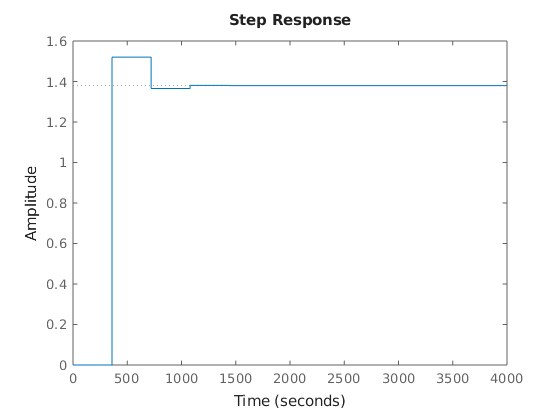
\includegraphics[width=0.5\linewidth]{images/resp2g.png}
			\label{fig:resposta_g}
		\end{figure}


\section{Problema 3}
A figura 3 mostra o sistema de controle de posição de uma junta de um braço robótico.
\begin{figure}[H]
	\centering
	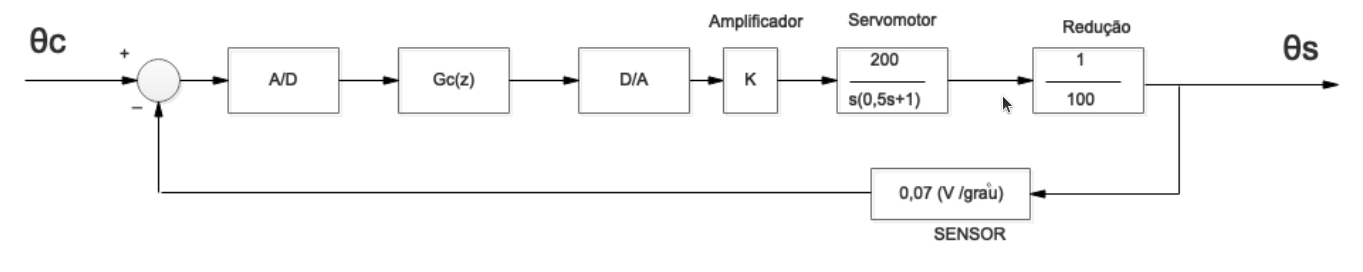
\includegraphics[width=0.9\linewidth]{images/planta_problema3}
	\caption{Sistema de controle de posição de uma junta de braço robótico}
	\label{fig:plantaproblema3}
\end{figure}

\subsection{Função de transferência de malha fechada}
Admitindo $T = 0,1$ s, $Gc(z) = 1,0$ e $K=2,4$ é necessário inicialmente realizar a conversão do controlador junto com os conversores para o domínio s, para isso é utilizado o segurador de ordem zero.
	\begin{equation}
		\left.
		\begin{array}{c}
			\displaystyle G_{SO}(s) = \frac{\displaystyle \frac{2}{T}}{s+\displaystyle\frac{2}{T}} = \frac{\displaystyle \frac{2}{0,1}}{s+\displaystyle\frac{2}{0,1}} = \frac{20}{s+20}
		\end{array}
		\right.
		\quad 
	\end{equation}
	
	Sendo assim o diagrama de blocos fica como mostra a figura \ref{img:gso}.

	\begin{figure}[H]
	    \centering
	    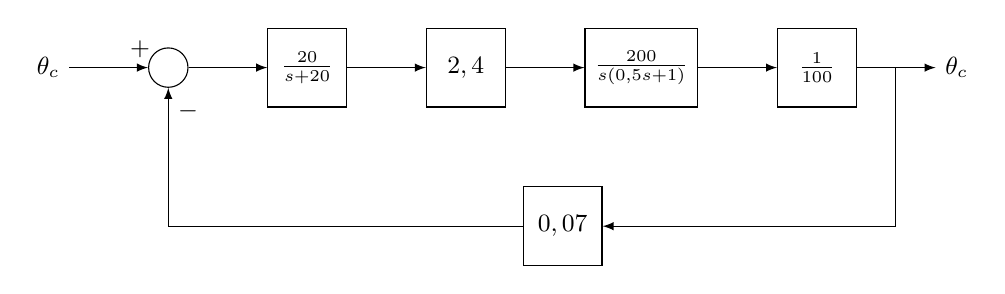
\begin{tikzpicture}[
	        block/.style={draw, rectangle, minimum width=1cm, minimum height=1cm, align=center},
	        sum/.style={draw, circle, node distance=1cm, inner sep=1pt, minimum size=0.5cm},
	        node distance=1cm, >=latex]
	        
	        % Nós do diagrama
	        \node (sum) [sum] {};  % Subtrator
	        \node (Gso) [block, right=of sum] {\small$\frac{20}{s+20}$};
	        \node (k) [block, right=of Gso] {\small$2,4$};   
	        \node (Gs) [block, right=of k] {\small $\frac{200}{s(0,5s+1)}$};
	        \node (red) [block, right=of Gs] {\small $\frac{1}{100}$};
	        \node (sensor) [block, below=of Gs, xshift=-1cm] {\small $0,07$};	        
	        
	        % Nós de entrada e saída
	        \node (angleIn) [left=of sum] {\small$\theta_c$};
	        \node (angleOut) [right=of red] {\small$\theta_c$};
	        
	        
%	        % Conexões
	        \draw[->] (angleIn) -- node[pos=0.9, above] {\small$+$} (sum.west);
	        
	        \draw[->] (sum) -- (Gso);
	        \draw[->] (Gso) -- (k);
	        \draw[->] (k) -- (Gs);
	        \draw[->] (Gs) -- (red);
	        \draw[->] (red) -- (angleOut);
	        
	        
	   		\draw[->] (red) -- ++(1, 0) |- (sensor);
	        \draw[->] (sensor) -| node[pos=0.85, above, xshift=2.5mm] {\small$-$} (sum.south);
	        
	        
%	        \node (fb) [coordinate, below=of Gs] {};
%			\draw[->] (red) -- ++(1, 0) |- (sum) -| node[pos=0.85, above, xshift=2.5mm] {\small$-$} (sum) ;
	    \end{tikzpicture}
	    \caption{Diagrama de blocos de uma junta de braço robótico}
	    \label{img:gso}
	\end{figure}
	
	Dessa forma a função de transferência de malha aberta será:
	\begin{equation}
		\left.
		\begin{array}{c}
			\displaystyle G_{c}(s) = \frac{20 \cdot 2,4 \cdot 200}{(s+20) \cdot (0,5s^2+s)\cdot 100} = \frac{96}{0,5s^3 + 11s^2 + 20s}
		\end{array}
		\right.
		\quad 
	\end{equation}
	
	E a função de malha fechada será:
	
	
	\begin{equation}
		\left.
		\begin{array}{c}
			\displaystyle G(s) = \frac{\displaystyle \frac{96}{0,5s^3 + 11s^2 + 20s}}{1 + \displaystyle \frac{6,72}{0,5s^3 + 11s^2 + 20s}\cdot 0,07} = \frac{192}{s^3 + 22s^2 +40s + 13,44} \rightarrow \\[30pt]
			
			 \rightarrow  \displaystyle G(s) = \frac{0,529}{s+20,04} + \frac{9,057}{s+0,44} - \frac{9,586}{s+1,52}
		\end{array}
		\right.
		\quad 
	\end{equation}
	
	A partir dessa equação e utilizando o software MATLAB resultou na seguinte função de transferência.
	
	\begin{equation}
		\left.
		\begin{array}{c}
			\displaystyle G(z) = \frac{0.011(z+1)^3}{(z-0,957)(z-0,8586)(z+0.00093)}
		\end{array}
		\right.
		\quad 
	\end{equation}
	
	Outra maneira de se obter a função de transferência de malha fechada é utilizando o H(z) assim como mostrado no Problema 2.
	
	\subsection{Faixa de tensão no sensor}
		Admitindo que o angulo de saída deve ficar entre $\pm135$ é possível obter a faixa de tensão na saída do sensor como mostra a equação abaixo.
		
		\begin{equation}
			\left.
			\begin{array}{c}
				\displaystyle \Delta V = (135 - (-135)) * 0,07 \rightarrow \Delta V = 18,9V
			\end{array}
			\right.
			\quad 
		\end{equation}
		
		Dependendo de qual a escolha da referência o intervalo de valores pode mudar, para esse exercício foi admitido que $0^\circ = 0V$ então o intervalo de valores será $\pm 9,45$.
		
	\subsection{Faixa de tensão do conversor A/D}
		Analisando a figura \ref{fig:plantaproblema3} é possível observar que a entrada do conversor A/D é também o erro do sistema, para encontrar qual a faixa de tensão desse erro pode-se analisar os dois extremos, quando a referência está em $135^\circ$ e a saída esta em $-135^\circ$  e vice-versa.
		
		
		\begin{equation}
			\left.
			\begin{array}{c}
				\displaystyle 135*0,07 - (-135*0,07) = 18,9V \\[10pt]
				\displaystyle -135*0,07 - 135*0,07 = -18,9V 
			\end{array}
			\right.
			\quad 
		\end{equation}
		
		Portanto a faixa de tensão do conversor A/D será de $\pm18,9V$ (37,8V).
		
\end{document}